\subsection{Hybrid MoE}
\label{subsec:hybridmoe}

The Nemotron 3 family of models utilize a hybrid Mamba-Transformer MoE architecture. This architecture is chosen with inference efficiency in mind, particularly for reasoning workloads, but also provides better or on-par accuracy compared to standard Transformers~\citep{waleffe2024empiricalstudymambabasedlanguage, nvidia2025nemotronhfamilyaccurateefficient, basant2025nvidia}. Specifically, rather than interleaving mixture-of-expert (MoE) layers with expensive self-attention layers---which need to attend over a linearly increasing KV Cache during generation---Nemotron 3 models predominantly interleave MoE layers with cheaper Mamba-2 layers~\citep{dao2024transformersssmsgeneralizedmodels}---which require storing only a constant state during generation. Only a select few attention layers are included in Nemotron 3 models. For example, we show the layer pattern for Nemotron Nano 3 in Figure~\ref{fig:layer-pattern}.

\begin{figure}[!t]
\centering
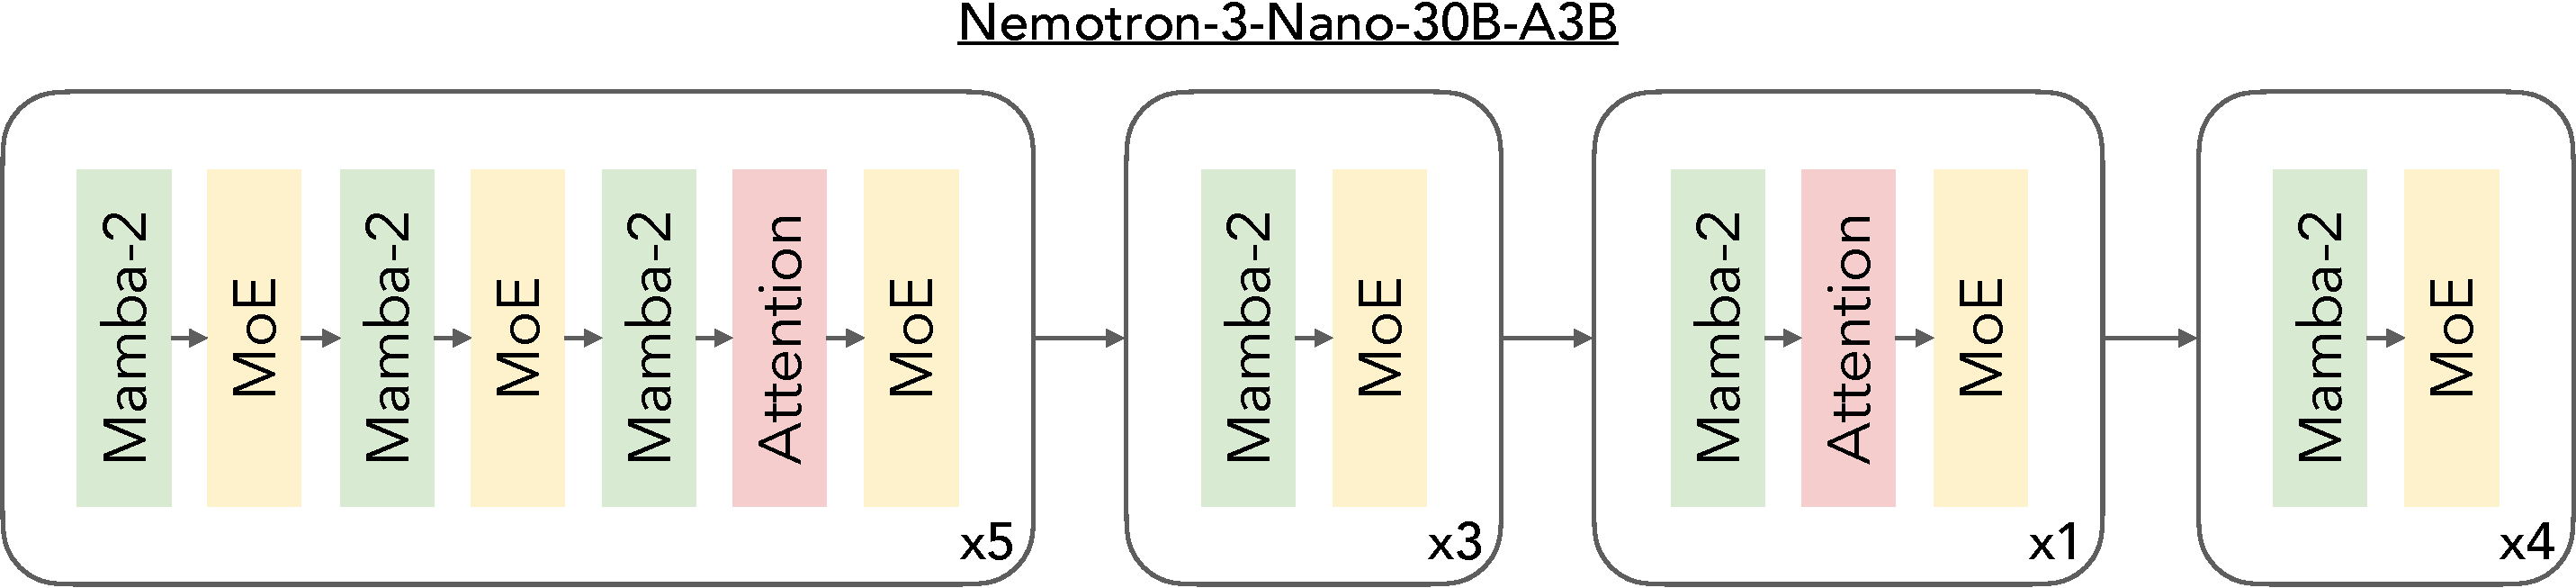
\includegraphics[width=0.9\linewidth]{figures/pattern.pdf}
\caption{Nemotron 3 models (e.g., Nemotron Nano 3) leverage a hybrid Mamba-Transformer MoE architecture consisting predominantly of interleaved Mamba-2 and MoE layers, with a select few self attention layers.}
\label{fig:layer-pattern}
\end{figure}

\begin{figure}[t]
    \centering
    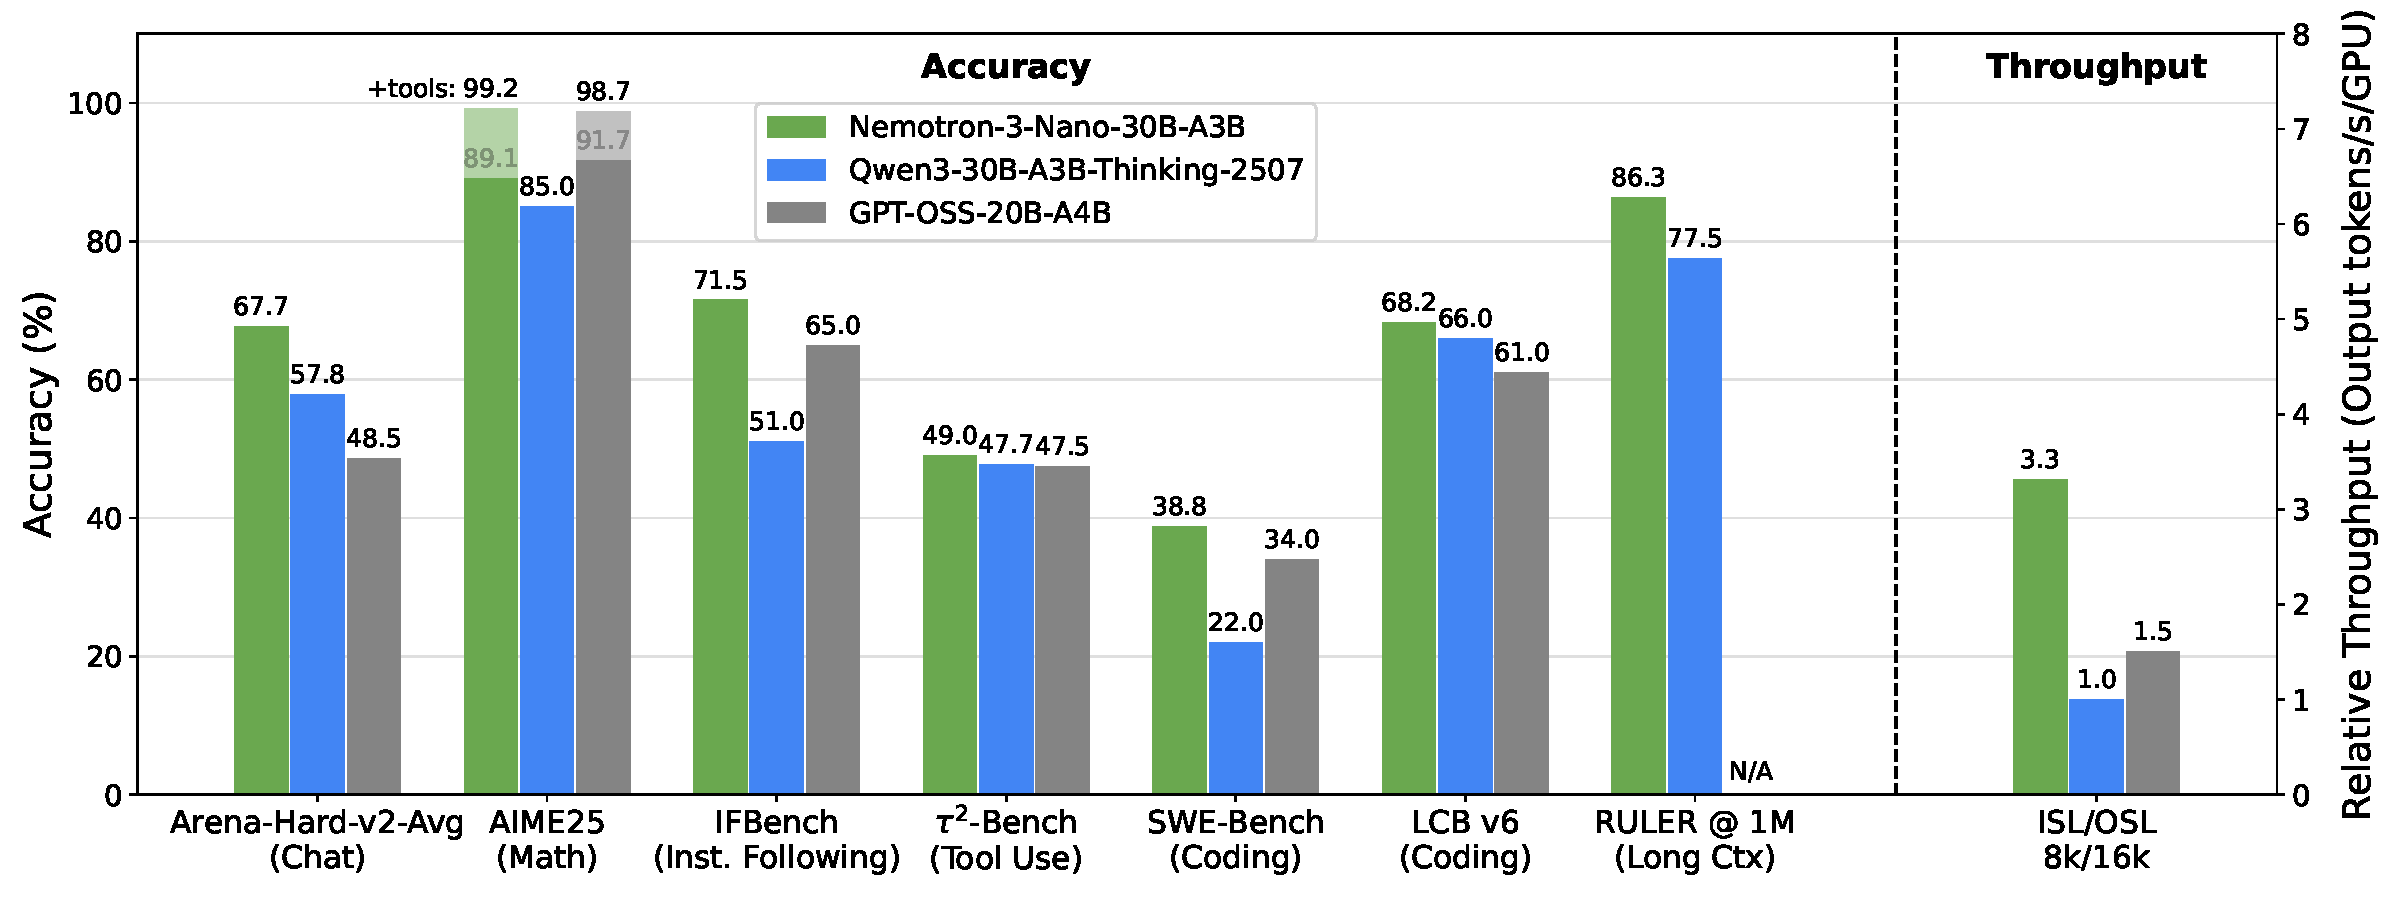
\includegraphics[width=\linewidth]{figures/nanov3_introfig.pdf}
    \caption{The hybrid Mamba-Transformer MoE architecture used by Nemotron 3 models can achieve state-of-the-art accuracy on leading reasoning benchmarks and ultra-long-context tasks while providing throughput improvements over similarly sized Transformer MoEs. For details, please see the Nemotron Nano 3 technical report. 
    % \todo{Change AIME tool numbers}
    }
    \label{fig:nanov3}
\end{figure}

By minimizing expensive self-attention layers, Nemotron 3 models can achieve higher inference throughput compared to similarly-sized Transformer MoEs for common reasoning workloads (e.g., 8k input sequence length / 16k output sequence length). For example, Nemotron 3 Nano 30B-A3B achieves 3.3$\times$ higher throughput compared to Qwen3-30B-A3B (Figure~\ref{fig:nanov3}), with further speedups at longer sequences. Yet the hybrid architecture can also achieve state-of-the-art accuracy, even on long-context lookup tasks (e.g., RULER on 1M token input sequences, see Figure~\ref{fig:nanov3}). 

Overall, the Nemotron 3 architecture leverages a balanced combination of mixture-of-expert layers that allow for sparse parameter scaling and lead to higher accuracy for a given compute budget, self-attention layers that enable high-fidelity all-to-all information routing, and Mamba-2 layers that enable sequence modeling with fixed inference-time computation and memory. 
